% Tento soubor nahraďte vlastním souborem s přílohami (nadpisy níže jsou pouze pro příklad)
% This file should be replaced with your file with an appendices (headings below are examples only)

% Umístění obsahu paměťového média do příloh je vhodné konzultovat s vedoucím
% Placing of table of contents of the memory media here should be consulted with a supervisor
%\chapter{Obsah přiloženého paměťového média}

%\chapter{Manuál}

%\chapter{Konfigurační soubor} % Configuration file

%\chapter{RelaxNG Schéma konfiguračního souboru} % Scheme of RelaxNG configuration file

%\chapter{Plakát} % poster


\chapter{PIR signal recording}
\label{appendix:PIRSignal}

The movements that data shows were prepared in several directions
and the type of movement can be read from the figure captions.

The trajectories are concentred circles with sensor in center and radius values $3~m$, $6~m$, $9~m$ and $12~m$.
The direction is either left-to-right (LR) or right-to-left (RL).
The workplace is shown in the figure \ref{fig:measurement}.
\footnote{For example {\it 6m\_RL} is movement $6~m$ from sensor right-to-left.}
The movement was recorded multiple times.

\begin{figure}[!ht]
\begin{center}

\includegraphics[width=0.25\textwidth]{obrazky-figures/measurement.png}
\caption{Measurement workplace.\label{fig:measurement}}
\end{center}
\end{figure}

Other cases are recorded as well: person walking towards ({\it C\_BF})
or walking away ({\it C\_FB}) from the sensor and no movement ({\it E}). 

\begin{figure}[!ht]
\begin{center}
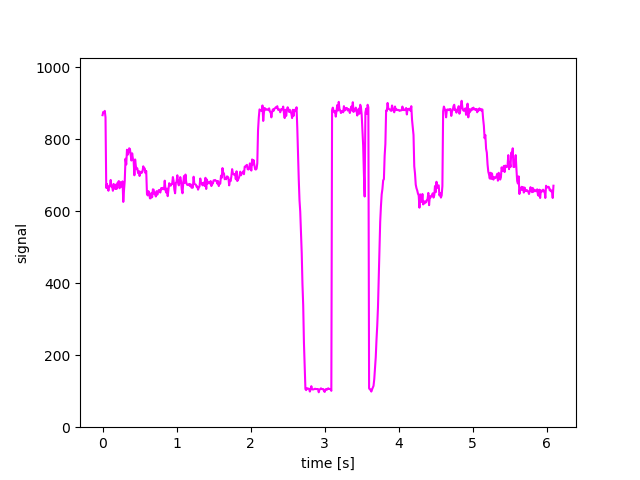
\includegraphics[width=0.3\textwidth]{../data/3m_LR/3m_LR_1.png}
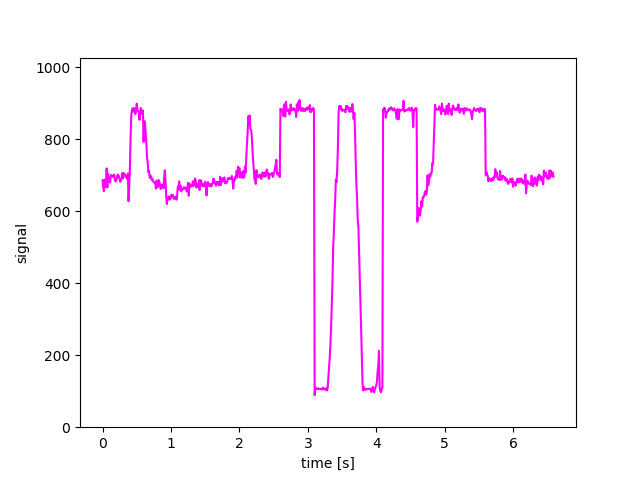
\includegraphics[width=0.3\textwidth]{../data/3m_LR/3m_LR_2.png}
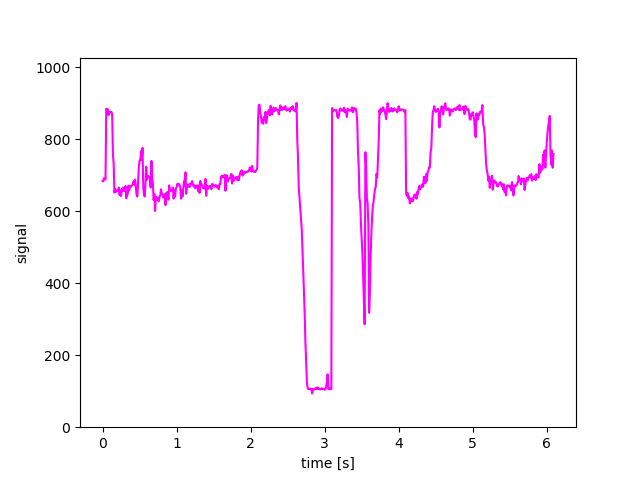
\includegraphics[width=0.3\textwidth]{../data/3m_LR/3m_LR_3.png}
\caption{3m\_LR.\label{fig:3m_LR}}
\end{center}
\end{figure}

\begin{figure}[!ht]
\begin{center}
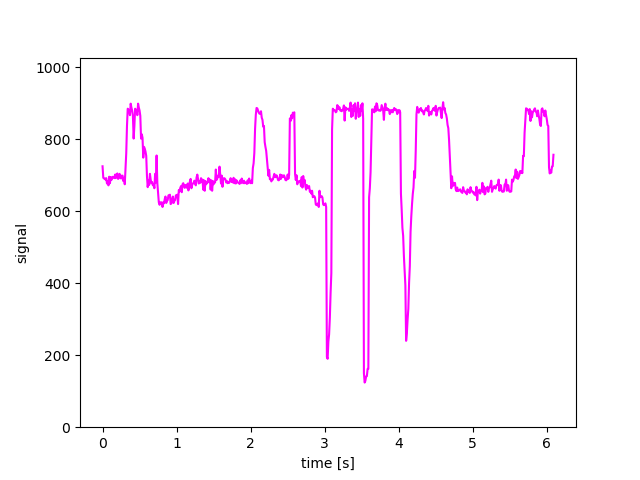
\includegraphics[width=0.3\textwidth]{../data/3m_RL2/3m_RL2_1.png}
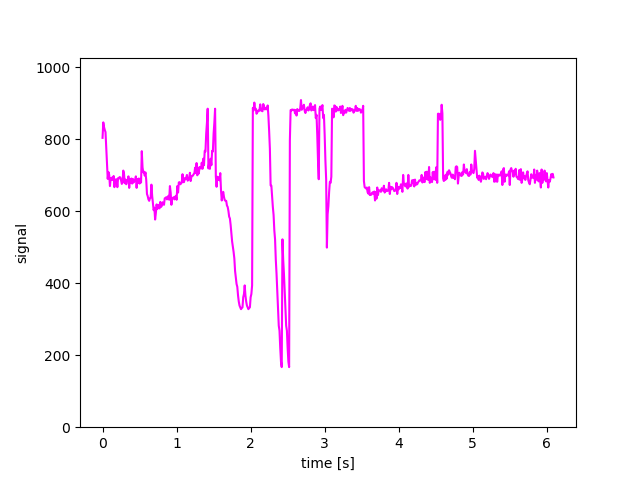
\includegraphics[width=0.3\textwidth]{../data/3m_RL2/3m_RL2_2.png}
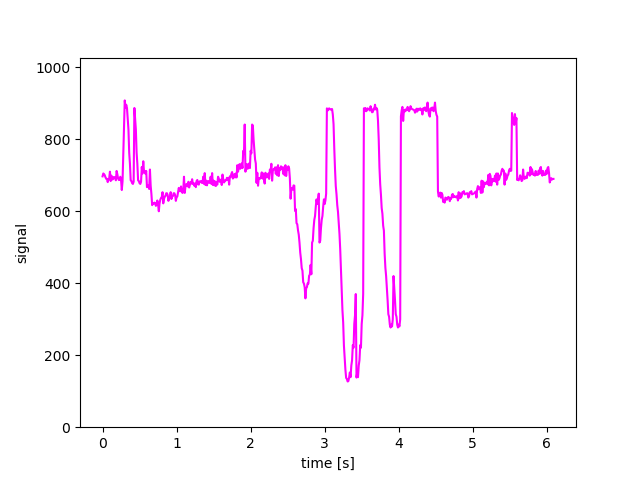
\includegraphics[width=0.3\textwidth]{../data/3m_RL2/3m_RL2_3.png}
\caption{3m\_RL.\label{fig:3m_RL}}
\end{center}
\end{figure}

\begin{figure}[!ht]
\begin{center}
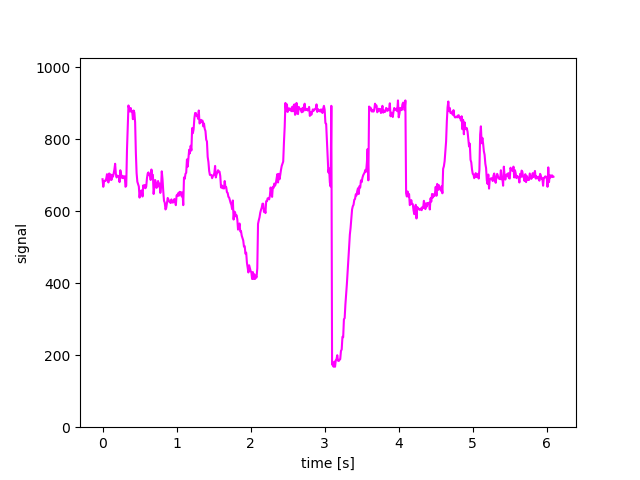
\includegraphics[width=0.3\textwidth]{../data/6m_LR/6m_LR_1.png}
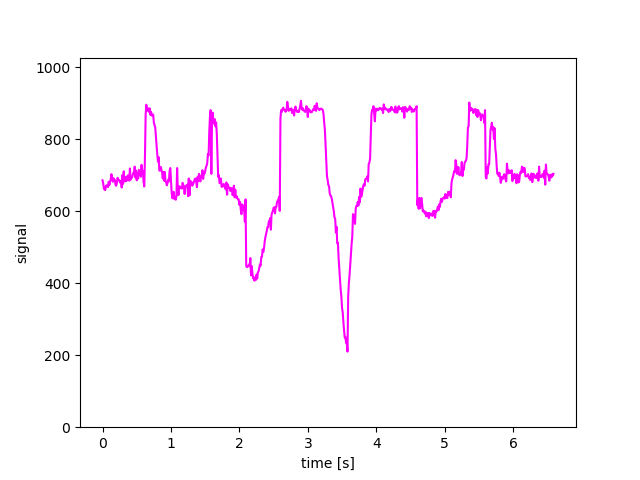
\includegraphics[width=0.3\textwidth]{../data/6m_LR/6m_LR_2.png}
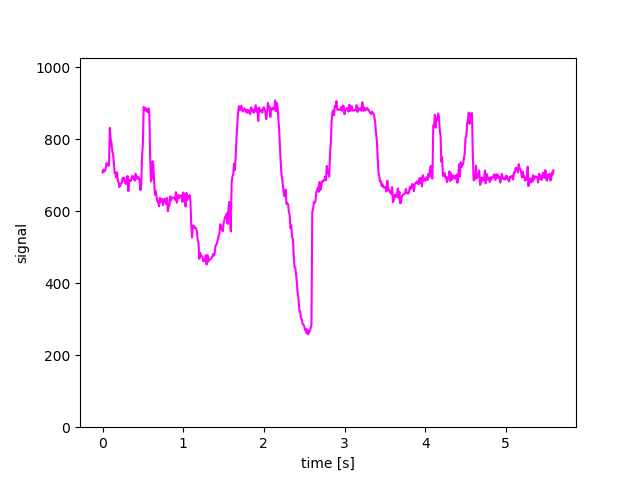
\includegraphics[width=0.3\textwidth]{../data/6m_LR/6m_LR_3.png}
\caption{6m\_LR.\label{fig:6m_LR}}
\end{center}
\end{figure}

\begin{figure}[!ht]
\begin{center}
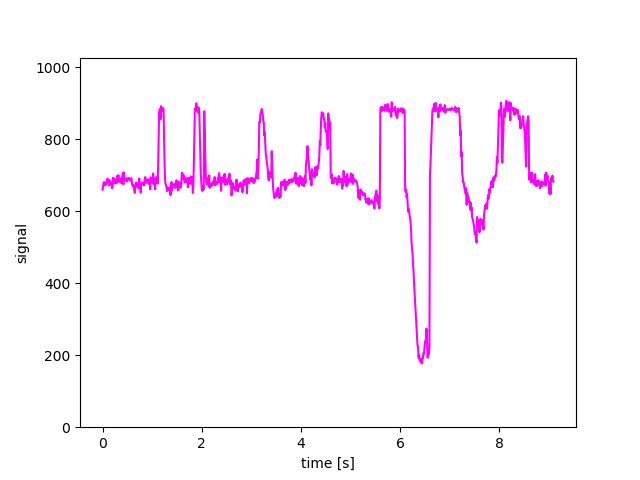
\includegraphics[width=0.3\textwidth]{../data/6m_RL/6m_RL_1.png}
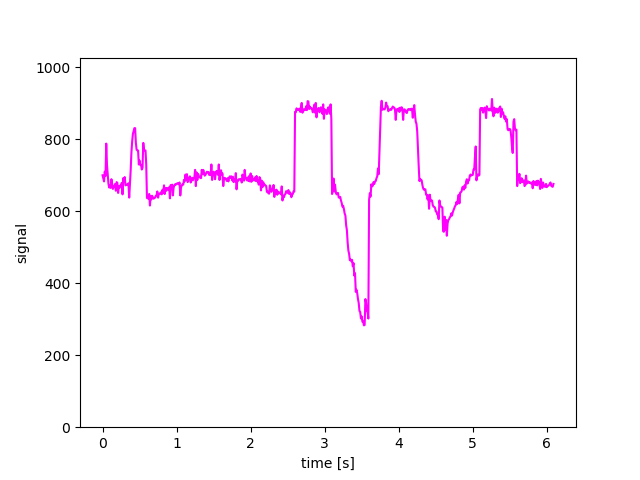
\includegraphics[width=0.3\textwidth]{../data/6m_RL/6m_RL_2.png}
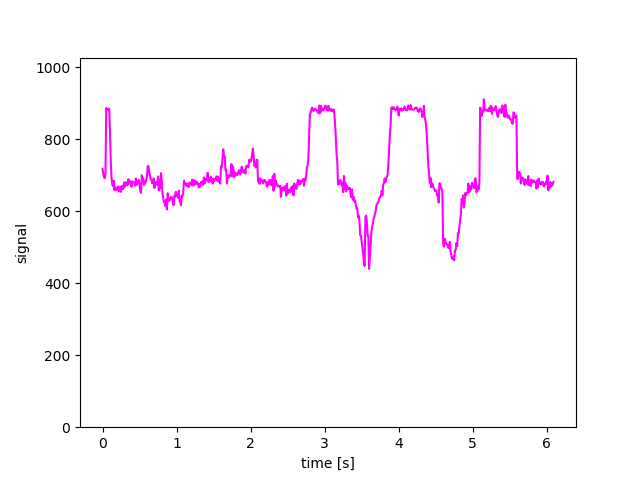
\includegraphics[width=0.3\textwidth]{../data/6m_RL/6m_RL_3.png}
\caption{6m\_RL.\label{fig:6m_RL}}
\end{center}
\end{figure}


\begin{figure}[!ht]
\begin{center}
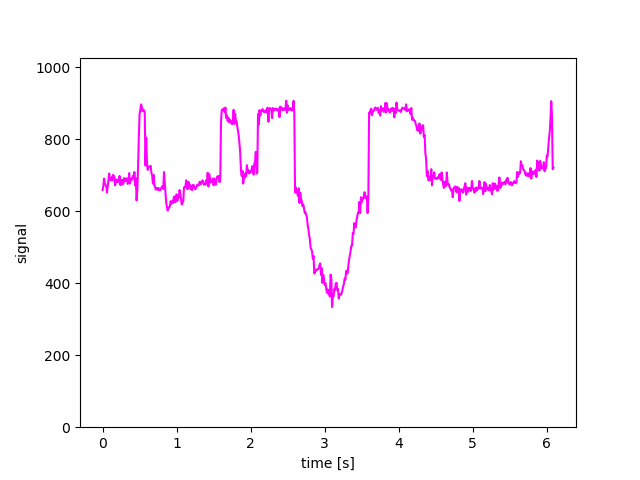
\includegraphics[width=0.32\textwidth]{../data/9m_LR/9m_LR_1.png}
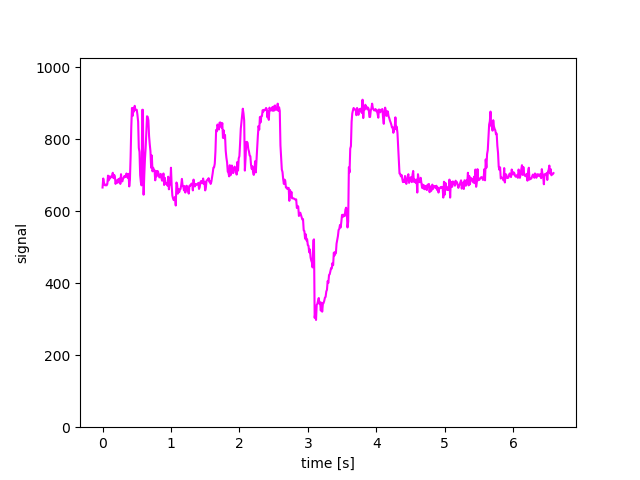
\includegraphics[width=0.32\textwidth]{../data/9m_LR/9m_LR_2.png}
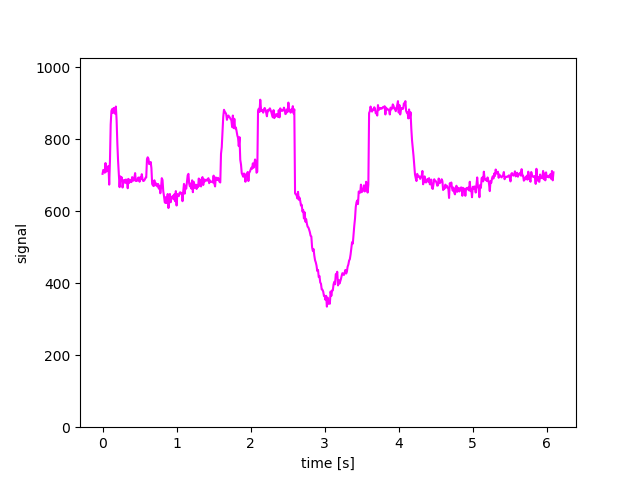
\includegraphics[width=0.32\textwidth]{../data/9m_LR/9m_LR_3.png}
\caption{9m\_LR.\label{fig:9m_LR}}
\end{center}
\end{figure}

\begin{figure}[!ht]
\begin{center}
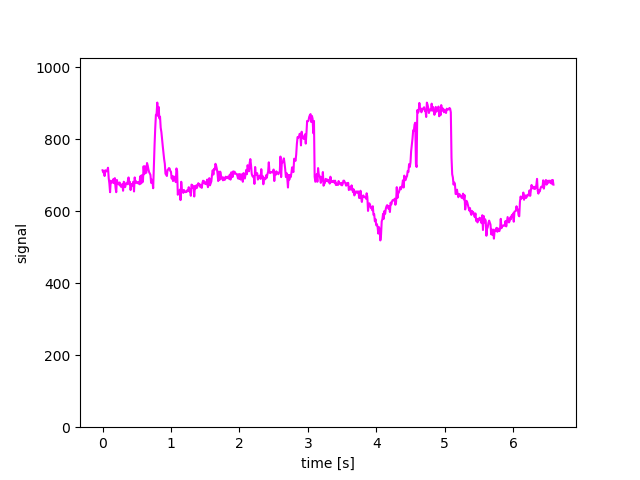
\includegraphics[width=0.3\textwidth]{../data/9m_RL/9m_RL_1.png}
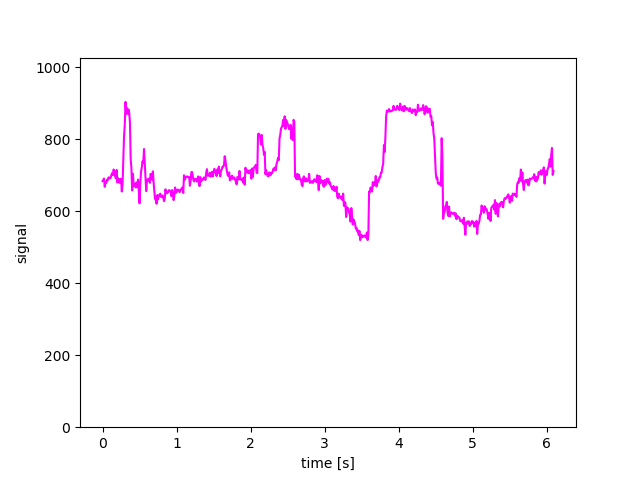
\includegraphics[width=0.3\textwidth]{../data/9m_RL/9m_RL_2.png}
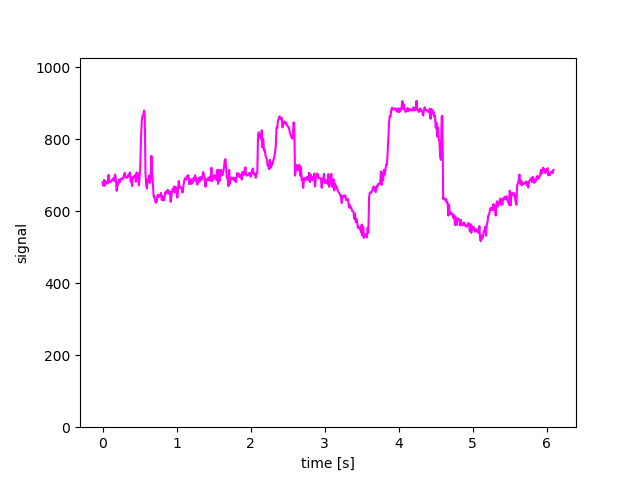
\includegraphics[width=0.3\textwidth]{../data/9m_RL/9m_RL_3.png}
\caption{9m\_RL.\label{fig:9m_RL}}
\end{center}
\end{figure}

\begin{figure}[!ht]
\begin{center}
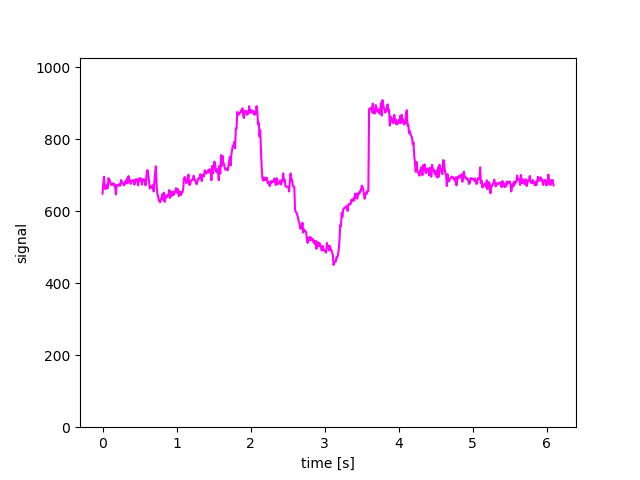
\includegraphics[width=0.3\textwidth]{../data/12m_LR/12m_LR_1.png}
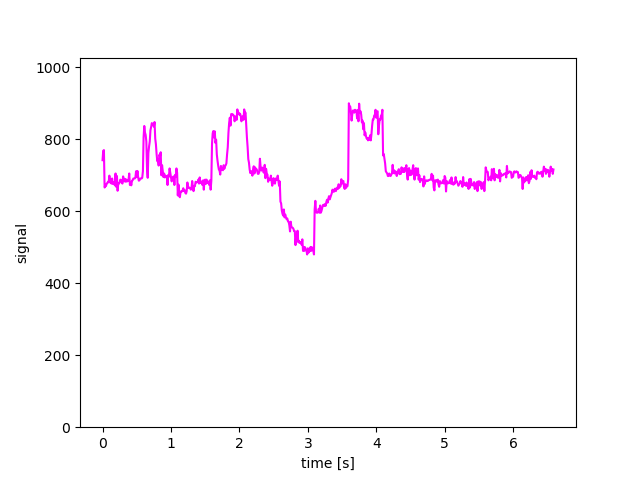
\includegraphics[width=0.3\textwidth]{../data/12m_LR/12m_LR_2.png}
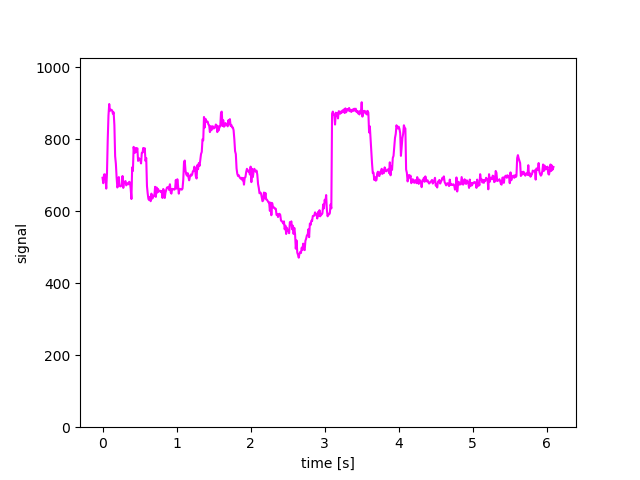
\includegraphics[width=0.3\textwidth]{../data/12m_LR/12m_LR_3.png}
\caption{12m\_LR.\label{fig:12m_LR}}
\end{center}
\end{figure}

\begin{figure}[!ht]
\begin{center}
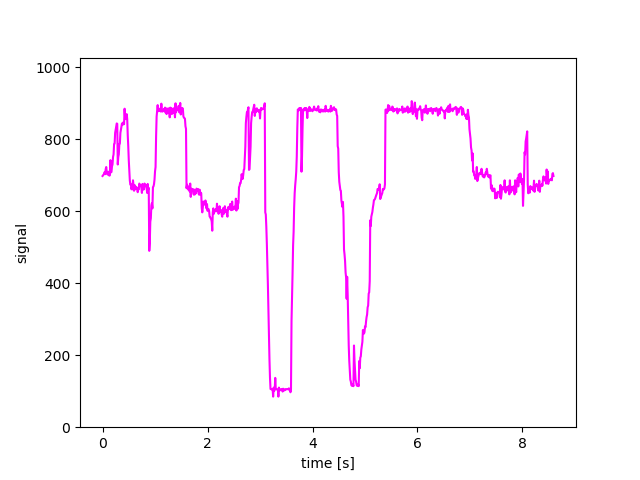
\includegraphics[width=0.3\textwidth]{../data/C_BF/C_BF_2.png}
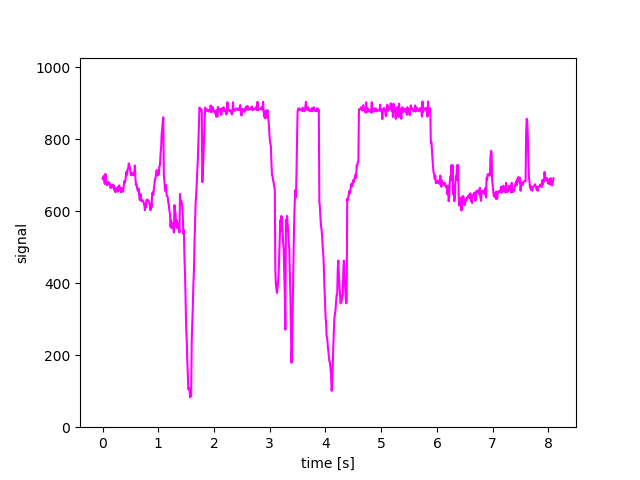
\includegraphics[width=0.3\textwidth]{../data/C_BF/C_BF_3.png}
\caption{C\_BF.\label{fig:C_BF}}
\end{center}
\end{figure}

\begin{figure}[!ht]
\begin{center}
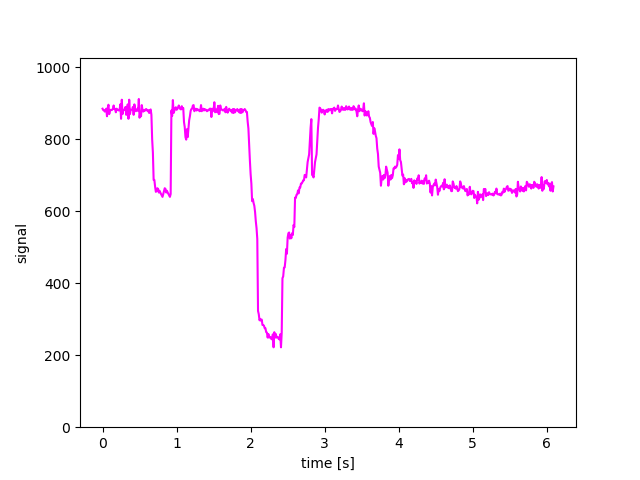
\includegraphics[width=0.3\textwidth]{../data/C_FB/C_FB_2.png}
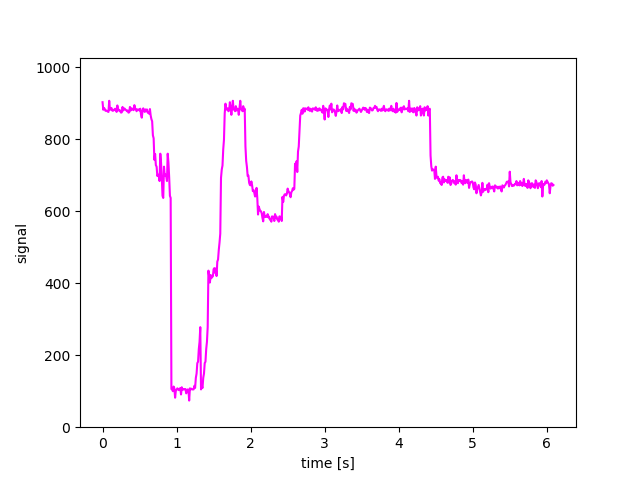
\includegraphics[width=0.3\textwidth]{../data/C_FB/C_FB_3.png}
\caption{C\_FB.\label{fig:C_FB}}
\end{center}
\end{figure}

\begin{figure}[!ht]
\begin{center}
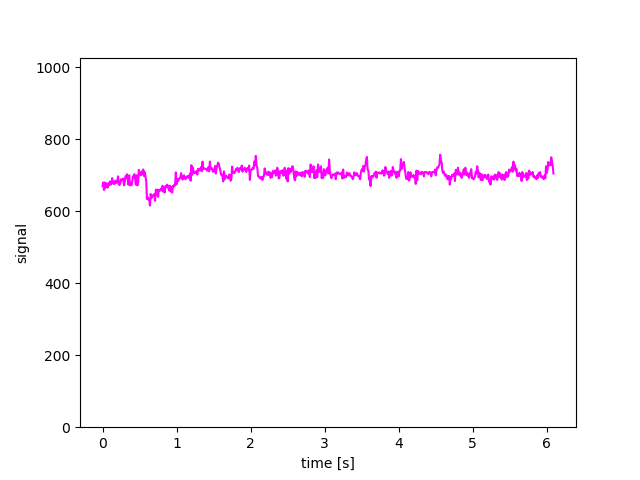
\includegraphics[width=0.3\textwidth]{../data/E2/E2_2.png}
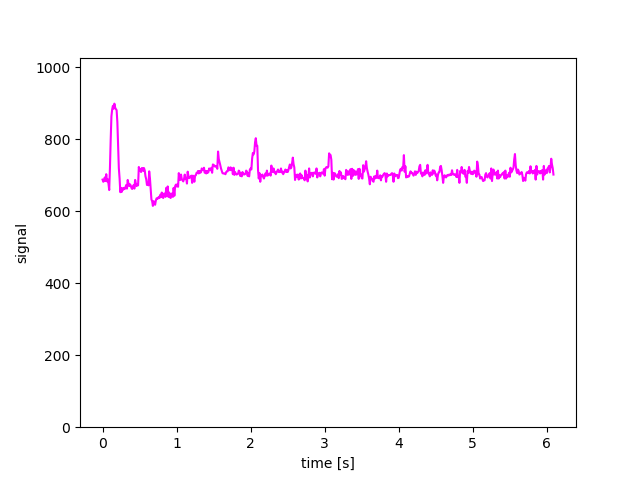
\includegraphics[width=0.3\textwidth]{../data/E2/E2_3.png}
\caption{E.\label{fig:C_FB}}
\end{center}
\end{figure}


%\begin{subequations}
%\begin{equation}
%    \alpha_A = \frac{2b_A}{r} = \frac{5}{11} = \underline{0.4545}
%\end{equation}
%\begin{equation}
%    \alpha_B = \frac{2b_A + 2b_B}{r} = \frac{5 + 10}{11} = \underline{1.3636}
%\end{equation}
%\begin{equation}
%    \alpha_C = \frac{2b_A + 2b_B + 2b_C}{r} = \frac{5 + 10 + 8}{11} = \underline{2.0909}
%\end{equation}
%\end{subequations}
%\begin{subequations}
%\begin{equation}
%    \varphi_1 = \frac{\alpha_C - \alpha_B}{2} = \frac{2.0909 - 1.3636}{2} = 0.36365
%\end{equation}
%\begin{equation}
%    \varphi_2 = \frac{\alpha_B - \alpha_A}{2} = \frac{1.3636 - 0.4545}{2} = 0.45455
%\end{equation}
%\begin{equation}
%    \varphi_3 = \frac{\alpha_A}{2} = \frac{0.4545}{2} = 0.22725
%\end{equation}
%\end{subequations}

%During the movement around the sensor with circular trajectory of radius $r_X$,
%the sectors are being crossed in the order $\varphi_1$, $\varphi_2$, $\varphi_3$,
%$\varphi_3^{'}$, $\varphi_2^{'}$, $\varphi_1^{'}$. The length of a sector $l$ is

%\begin{equation}
%  l = \varphi r
%\end{equation}

%The measurement was done in a room with width $w = 7.63~m$, $w_R = 4.25~m$ on the right
%and $w_L = 3.38~m$ from the left. The radiuses of circular trajectories were $3~m$, $6~m$, $9~m$ and $12~m$.

%To calculate maximal possible angle equation at figure \ref{fig:maxangle} can be used, $w$ is a distance of
%the sensor and a side wall, $r$ is a distance of the object we want to calculate the maximal angle of.

%\begin{figure}[ht!]
%\begin{equation}
%\varphi_{max}(w, r) = \text{min}(\frac{\alpha_C}{2}, 
%  \begin{cases}
%    \text{arcsin}(\frac{w}{r}) & \frac{w}{r} \in (0 ; 1) \\ 
%    \infty                      & \text{otherwise}
%  \end{cases}
%)
%\end{equation}
%\caption{Instantaneous maximal angle. \label{fig:maxangle}}
%\end{figure}

%\begin{subequations}
%\begin{equation}
%\varphi_{max}(3.38~m, 3~m) = \text{min}(\frac{2.0909}{2}, \infty) =  1.04545
%\end{equation}
%\begin{equation}
%\varphi_{max}(4.25~m, 3~m) = \text{min}(1.04545, \infty) =  1.04545
%\end{equation}
%\end{subequations}

%\begin{subequations}
%\begin{equation}
%\varphi_{max}(3.38~m, 6~m) = \text{min}(1.04545, \text{arcsin}(\frac{3.38}{6})) = 0.59841
%\end{equation}
%\begin{equation}
%\varphi_{max}(4.25~m, 6~m) = \text{min}(1.04545, \text{arcsin}(\frac{4.25}{6})) = 0.78713
%\end{equation}
%\end{subequations}

%\begin{subequations}
%\begin{equation}
%\varphi_{max}(3.38~m, 9~m) = \text{min}(1.04545, \text{arcsin}(\frac{3.38}{9})) = 0.385
%\end{equation}
%\begin{equation}
%\varphi_{max}(4.25~m, 9~m) = \text{min}(1.04545, \text{arcsin}(\frac{4.25}{9})) = 0.49181
%\end{equation}
%\end{subequations}



%\begin{subequations}
%\begin{equation}
%\varphi_{max}(3.38~m, 12~m) = \text{min}(1.04545, \text{arcsin}(\frac{3.38}{12})) = 0.28553
%\end{equation}
%\begin{equation}
%\varphi_{max}(4.25~m, 12~m) = \text{min}(1.04545, \text{arcsin}(\frac{4.25}{12})) = 0.36202
%\end{equation}
%\end{subequations}

%This means, that walking around the circle should generate signal that will be scaled with
%the distance of the object from the sensor.


\newpage
\chapter{REST API of MCU HTTP server}
\label{appendix:mcu_restapi}

The MCU runs a REST API, that can configure it. The API includes following options:

\begin{table}[h!]
    \begin{tabular}{|l|l|} \hline
        \textbf{Resource} & \textbf{Description} \\ \hline
        \texttt{/} & Welcome page. \\ \hline
        \texttt{/config} & Configuration of module. \\ \hline
        \texttt{/config/mcast}  & Configuration of multicast channel. \\ \hline
        \texttt{/config/sample} & Configuration of sampling. \\ \hline
        \texttt{/config/send}   & Configuration of sending. \\ \hline
        \texttt{/log}         & Logs. \\ \hline
    \end{tabular}
    \caption{REST API resources overview.}
\end{table}

\section*{Resources}

\paragraph{\texttt{/config/mcast}}
Configures the multicast channel.
\begin{itemize}
    \item[] \texttt{enabled} Enables/disables sending. Defaultly enabled.
    \item[] \texttt{address} Sets multicast channel address. Defaultly \texttt{224.0.0.1}.
    \item[] \texttt{port}    Sets multicast channel port. Defaultly \texttt{1234}.
\end{itemize}

\paragraph{\texttt{/config/sample}}
Configures the sampling.
\begin{itemize}
    \item[] Exactly one of the parameters must be present (ignored otherwise):
    \item[] \texttt{frequency} Sets sampling frequency, subsequently changing sampling period (\ref{eq:period_frequency}) and segment size (\ref{eq:segmentsize}). Defaultly $100$.
    \item[] \texttt{period}    Sets sampling period, subsequently changing sampling frequency (\ref{eq:period_frequency}) and segment size (\ref{eq:segmentsize}). Defaultly $0.01$.
\end{itemize}

\paragraph{\texttt{/config/send}}
Configures the sending.
\begin{itemize}
    \item[] Exactly one of the parameters must be present (ignored otherwise):
    \item[] \texttt{frequency} Sets sampling frequency, subsequently changing sampling period (\ref{eq:period_frequency}) and segment size (\ref{eq:segmentsize}). Defaultly $0.5$.
    \item[] \texttt{period}    Sets sampling period, subsequently changing sampling frequency (\ref{eq:period_frequency}) and segment size (\ref{eq:segmentsize}). Defaultly $2$.
    \item[] \texttt{N}         Sets segment size, subsequently changing sampling frequency and period (\ref{eq:period_frequency}). Defaultly $200$.
\end{itemize}

The segment size must lay between 10 and 1024. If set value causes invalid value of segment size,
request will be ignored. The conversion to segment size $N$ is shown in the formula \ref{eq:segmentsize}.

\begin{subequations}
\begin{equation}
f = T^{-1}
\end{equation}
\begin{equation}
T = f^{-1}
\end{equation}
%\caption{Conversion period $T$ to frequency $f$ and vice versa.}
\label{eq:period_frequency}
\end{subequations}

\begin{subequations}
\begin{equation}
N = T_{send}T_s^{-1}
\end{equation}
\begin{equation}
N = f_sf_{send}^{-1}
\end{equation}
\begin{equation}
N = f_sT_{send}
\end{equation}
\begin{equation}
N = (T_sf_{send})^{-1}
\end{equation}
%\caption{Computation of segment size $N$.}
\label{eq:segmentsize}
\end{subequations}


\paragraph{\texttt{/log}}

Shows last events of the sensor in a form of logs.





